\section{Logarithmic Functions}
\label{sec:log}

Logarithms are the inverse of exponential functions – they allow us to undo exponential functions and solve for the exponent. They are also commonly used to express quantities that vary widely in size.

\begin{definition}[Logarithms and Exponentials]
The {\bf logarithm function}\index{Function!logarithm} of {\bf base}\index{Base} $b$, written $\log_b(x)$, is the inverse of the {\bf exponential function}\index{Function!exponential} (base $b$), $b^x$.

This means the statement $b^a=c$ is equivalent to the statement $\log_b(c)=a$.
\end{definition}

\begin{theorem}[Properties of Logarithms\index{Properties of logarithms}: Inverse Properties]
If $b>0$ and $b\neq 1$, then:
  \begin{itemize}
    \item $\log_b(b^x)=x$ for all $x\in\R$;
    \item $b^{\log_b(x)}=x$ for all $x>0$.
  \end{itemize}
\end{theorem}

\begin{example}
Write these exponential equations as logarithmic equations:
\begin{enumerate}[label={\alph*)}]
  \item $2^3=8$
  \item $5^2=25$
  \item $10^{-4}=\dfrac{1}{10000}$
\end{enumerate}
\begin{solution}
\begin{enumerate}[label={\alph*)}]
  \item $2^3=8$ is equivalent to $\log_2(8)=3$.
  \item $5^2=25$ is equivalent to $\log_5(25)=2$.
  \item $10^{-4}=\dfrac{1}{10000}$ is equivalent to $\log_{10}\left(\dfrac{1}{10000}\right)=-4$.
\end{enumerate}
\end{solution}\end{example}
\begin{example}
  Solve $2^x=10$ for $x$.

\begin{solution}  By rewriting this expression as a logarithm, we get $x=\log_2(10)$.
\end{solution}\end{example}

While this does define a solution, and an exact solution at that, you may find it somewhat unsatisfying since it is difficult to compare this expression to the decimal estimate we made earlier. Also, giving an exact expression for a solution is not always useful–often we really need a decimal approximation to the solution. Luckily, this is a task calculators and computers are quite adept at. Unluckily for us, most calculators and computers will only evaluate logarithms of two bases. Happily, this ends up not being a problem, as we’ll see briefly.

\begin{definition}[Common and Natural Logarithms] These are by far the most frequently used logarithms.
  \begin{itemize}
    \item The {\bf common logarithm}\index{Logarithm!common} is the logarithm with base 10, and is typically written $\log(x)$.
    \item The {\bf natural logarithm}\index{Logarithm!natural} is the logarithm with base $e$, and is typically written $\ln(x)$.
  \end{itemize}
\end{definition}
\begin{example}
Evaluate $\log(1000)$ using the definition of the common logarithm.

\begin{solution}  $$10^x=1000 \enspace .$$
From this, we might recognize that 1000 is the cube of 10, i.e., $10^3$, so $x=3$.

We also can use the inverse property of logarithms  to write $\log_{10}(10^3)=3$.
\end{solution}\end{example}
\begin{table}[!ht]
\centering
\caption{Values of the common logarithm}
\begin{tabular}{ccc}
  \toprule
  $x$ & $x$ as an exponential	& $\log(x)$\\
  \midrule
  1000 & $10^3$ &	3\\
  100 &	$10^2$ &	2	\\
  10 &	$10^1$ &	1	\\
  1 &	$10^0$ &	0\\
	0.1 &	$10^{-1}$ &	$-1$\\
  0.01 &	$10^{-2}$ &	$-2$\\
  0.001 &	$10^{-3}$ &	$-3$\\
  \bottomrule
\end{tabular}
\end{table}

\begin{example}
Evaluate $\log(500)$ using your calculator or computer.

\begin{solution}  Using a computer or calculator, we can evaluate and find that $\log(500)\approx   2.69897$.
\end{solution}\end{example}

Another property provides the basis for solving exponential equations.

\begin{theorem}[Properties of Logarithms: Exponent Property]
$$\log_b(A^r)=r\log_b(A)$$
\end{theorem}

\begin{remark}[Solving exponential equations:] Here are steps to help you solve exponential equations by hand.
\begin{itemize}
  \item Isolate the exponential expressions when possible.
  \item Take the logarithm of both sides.
  \item Utilize the exponent property for logarithms to pull the variable out of the exponent.
  \item Use algebra to solve for the variable.
\end{itemize}
\end{remark}
\begin{example}
In the last section, we predicted the population (in billions) of India $t$ years after 2008 by using the function $f(t)=1.14(1+0.0134)^t$. If the population continues following this trend, when will the population reach 2 billion?

\begin{solution}  We need to solve for $t$ so that $f(t)=2$.
\begin{align*}
    2 &= 1.14(1.0134)^t&  &\mbox{Initial equation.}\\
    \dfrac{2}{1.14} &= 1.0134^t&  & \mbox{Divide by 1.14 to isolate the exponential expression.}\\
    \ln\left(\dfrac{2}{1.14}\right) &= \ln\left(1.0134^t\right)&  &\mbox{Take the logarithm of both sides of the equation.}\\
    \ln\left(\dfrac{2}{1.14}\right) &= t\cdot\ln(1.0134)& &\mbox{Apply the exponent property on the right side.}\\
    t &= \dfrac{\ln\left(\dfrac{2}{1.14}\right)}{\ln(1.0134)}& &\mbox{Divide both sides by } \ln(1.0134).\\
    t &\approx 42.23 \mbox{ years} & &
\end{align*}

If this growth rate continues, the model predicts the population of India will reach 2 billion about 42 years after 2008, or approximately in the year 2050.
\end{solution}\end{example}
\begin{example}
Solve $5e^{-0.3t}=2$ for $t$.

\begin{solution}  First we divide by 5 to isolate the exponential:
$$e^{-0.3t}=\frac{2}{5} \enspace .$$
Since this equation involves $e$, it makes sense to use the natural logarithm:

\begin{align*}
    \ln\left(e^{-0.3t}\right) &= \ln\left(\dfrac{2}{5}\right)& &\mbox{Take the natural logarithm of both sides.}\\
    -0.3t &= \ln\left(\dfrac{2}{5}\right)& &\mbox{Utilize the inverse property of logarithms.}\\
    t &= \dfrac{\ln\left(\dfrac{2}{5}\right)}{-0.3}&  &\mbox{Now divide by } -0.3.\\
    t &\approx 3.054& &\\
\end{align*}
\end{solution}\end{example}

In addition to solving exponential equations, logarithmic expressions are common in many physical situations.

\begin{example} The mass of a 300 gram sample of Indium-111 is $f(t) = 300\cdot 2^{-t/2.807}$ grams after $t$ days. How long will it take the sample to decay to 100 grams?

    \begin{solution} 
    \begin{align*}    
    100 &= 300\cdot 2^{-t/2.807}\\
      \dfrac{1}{3} &= 2^{-t/2.807} \\
    \log_2\left(\dfrac{1}{3}\right) &= \log_2(2^{-t/2.807}) \\
    \log_2(3^{-1}) &= \frac{-t}{2.807} \\
    -\log_2(3) &= \frac{-t}{2.807} \\
    t &= 2.807\cdot\log_2(3) \\
    &= 2.807\cdot\frac{\log(3)}{\log(2)} \approx 2.807\cdot\frac{0.477121}{0.301030}\\
    &\approx 4.449\text{ days}
    \end{align*}
\end{solution}\end{example}

\begin{example}
In chemistry, $pH$ is a measure of the acidity or basicity of a liquid. The $pH$ is related to the concentration of hydrogen ions, $[H^+]$, measured in moles per liter, by the equation
$$pH=-\log([H^+])$$
If a liquid has concentration of 0.0001 moles per liter, determine the pH. Determine the hydrogen ion concentration of a liquid with $pH$ of 7.

\begin{solution}  To answer the first question, we evaluate the expression $-\log(0.0001)$. While we could use our calculators for this, we do not really need them here, since we can use the inverse property of logarithms:
$$-\log(0.0001)=-\log(10^{-4})=-(-4)=4 \enspace .$$
To answer the second question, we need to solve the equation $7=-\log([H^+])$. Begin by isolating the logarithm on one side of the equation by multiplying both sides by $-1$: $-7=\log([H^+])$. Rewriting into exponential form yields the answer
$$[H^+]^{-7}=0.0000001 \mbox{ moles per liter.}$$
\end{solution}\end{example}

While we don't often need to sketch the graph of a logarithm, it is helpful to understand the basic shape.

\begin{theorem}[Graphical Features of the Logarithm]
  Graphically, given the function $g(x)=\log_b(x)$:
  \begin{itemize}
    \item The graph has a horizontal intercept at the point $(1, 0)$.
    \item The graph has a vertical asymptote at $x=0$.
    \item The graph is increasing and concave down.
    \item The domain of the function is $x>0$, or $(0,\infty)$ in interval notation.
    \item The range of the function is all real numbers ($\R$) or $(-\infty,\infty)$ in interval notation.
  \end{itemize}
\end{theorem}
When sketching a general logarithm with base b, it can be helpful to remember that the graph will pass through the points $\left(\dfrac{1}{b}, -1\right)$, $(1,0)$, and $(b,1)$.

To get a feeling for how the base affects the shape of the graph, examine the graphs below:

\begin{figure}[ht!]
\centering
  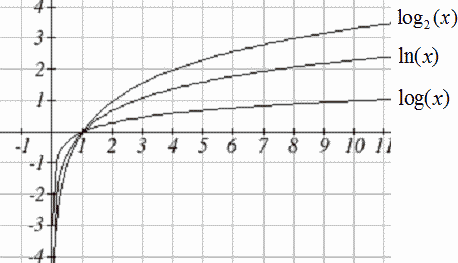
\includegraphics[width=0.5\textwidth]{img/chap1/sec1-8/image080.png}
\caption{Graphs of the Binary, Natural, and Common Logarithms}
\end{figure}

Another important observation made was the domain of the logarithm: $x>0$. Like the reciprocal and square root functions, the logarithm has a restricted domain which must be considered when finding the domain of a composition involving a logarithm.

\begin{example}
Find the domain of the function $f(x)=\log(5-2x)$.

\begin{solution}  The logarithm is only defined when the input is positive, so this function will only be defined when $5-2x>0$. Solving this inequality, $-2x>-5$, so $x<\frac{5}{2}$.

The domain of this function is $x<\frac{5}{2}$, or, in interval notation, $\left(-\infty,\frac{5}{2}\right)$.
\end{solution}\end{example}
